\section{Docker}
\sectionslide{Docker}
\begin{frame}
	\frametitle{Docker}
	
	\begin{columns}
		\column{.55\textwidth}
		\begin{itemize}
			\item Runtime and engine
			\item Building / managing of images / containers
			\item Distribution of images (Docker Hub)
			\item Interface to Windows and MacOS, different mechanisms
			\item (Orchestration of containers) swarm, \codi{docker-compose}
			\item Docker engine exists as open source, Docker Desktop and Docker Hub are developed by \myhref{https://www.docker.com/company}{Docker Inc.}
		\end{itemize}
		\column{.45\textwidth}
		\textbf{Docker is the most relevant container tool for us.}
		
		\vspace{.2cm}We will take a short tour of the most important \hervor{Docker concepts}:
		\begin{itemize}
			\item Running containers
			\item Building images with \codi{Dockerfile}s
			\item Docker registries (\myhref{https://hub.docker.com/}{Docker Hub}, company self-hosting solutions)
			\item Pushing / pulling images
			\item Docker volumes
		\end{itemize}
	\end{columns}
	
\end{frame}

\begin{frame}
	\frametitle{Code-along exercises}
	
	\centering
	
\includegraphics[width=3cm]{pics/codealong.png}
	
	\begin{itemize}
		\item Feel free to try out the commands presented on the next slides during the training!
		\item You need a \myhref{https://www.docker.com/products/docker-desktop}{Docker Desktop} installation (or \myhref{https://hub.docker.com/search?offering=community\&operating\_system=linux\&q=\&type=edition}{Docker Engine on Linux})
		\item As a preparation, clone  \myhref{https://github.com/scherbertlemon/docker-training}{github.com/scherbertlemon/docker-training}
	\end{itemize}
\end{frame}

\begin{frame}
	\frametitle{Container registries}
	\begin{block}{Container registries}
		... where prepared container images come from, if you do not build them based on your host system. They are usually organised in versioned image repositories.
	\end{block}
	\vspace{0.25cm}\begin{columns}[t]
		\column{.6\textwidth}
		\myhref{https://hub.docker.com}{Docker Hub} hosted by Docker Inc.
		\begin{itemize}
			\item Open registry where you can store your images in \textbf{repositories}
			\item Public repositories are free of charge
			\item Many \myhref{https://hub.docker.com/search?q=\&type=image\&image\_filter=official}{officially curated images}
		\end{itemize}
		
		\column{.4\textwidth}
		\myhref{}{Your company solution here}
		\begin{itemize}
			\item you might want to host your own registry
		\end{itemize}
	\end{columns}
    \vspace{0.5cm}\begin{itemize}
		\item Connect to a registry with \codi{docker login <url>}. If no URL, Docker Hub is the default.
		\item Generate an \hervor{Access Token} if possible and use it for login instead of your password.
	\end{itemize}
	
\end{frame}

\begin{frame}
	\frametitle{Images and Containers}
	\begin{columns}
		\column{.47\textwidth}
		\centering
			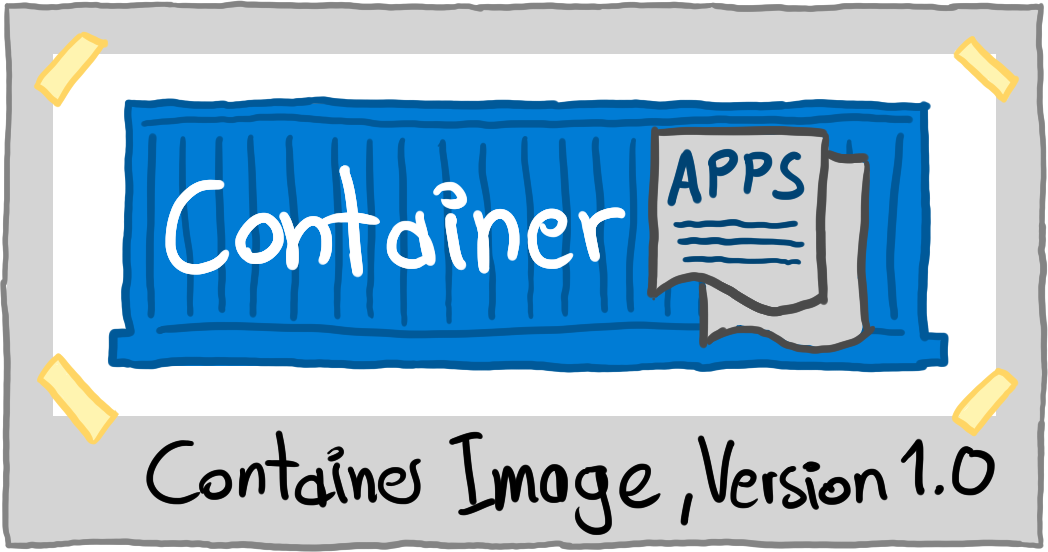
\includegraphics[width=.75\textwidth]{pics/container_image.png}
			
		\column{.47\textwidth}
		\centering
			
\includegraphics[width=.75\textwidth]{pics/container_large.png}
			
	\end{columns}
	\begin{columns}[t]
		\column{.47\textwidth}
		\centering
		\begin{block}{Image}
			Read only content of a container, e.g. file system, environment variables, metadata
		\end{block}
		\begin{itemize}
			\item Organized in \hervor{layers} ("differences")
			\item We usually \hervor{pull / push} images from / to \textbf{container registries}
		\end{itemize}
		
		\column{.47\textwidth}
		\centering
		\begin{block}{Container}
			Extracted image content plus writable layer, that can be run on the host OS.
		\end{block}
		\begin{itemize}
			\item We usually \hervor{run} processes in a container
			\item Changes to the file system exist as long as the container is not stopped and removed
		\end{itemize}
	\end{columns}
\end{frame}

\begin{frame}[fragile]
	\frametitle{Images and Containers}
	\begin{columns}
		\column{.47\textwidth}
		\centering
		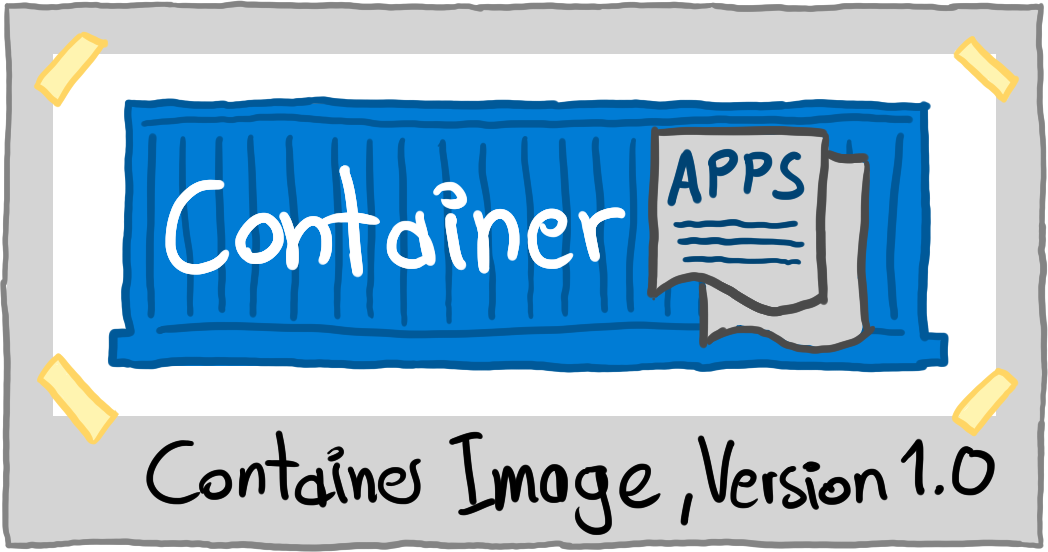
\includegraphics[width=.75\textwidth]{pics/container_image.png}
		
		\column{.47\textwidth}
		\centering
		
\includegraphics[width=.75\textwidth]{pics/container_large.png}
		
	\end{columns}
	\begin{columns}[t]
		\column{.47\textwidth}
		\begin{lstlisting}
# get the offical ubuntu image
docker pull ubuntu:focal
# check the local images
docker image ls
# check the properties of this image
docker image inspect ubuntu:focal
# remove the local image
docker image rm ubuntu:focal
		\end{lstlisting}
		
		\column{.5\textwidth}
		\begin{lstlisting}
# get an interactive shell in ubuntu
docker run -it --name ubu ubuntu:focal
# check the list of containers
docker container ls --all
# check the properties of ubu container
docker container inspect ubu
# remove stopped container
docker container rm ubu
		\end{lstlisting}
	\end{columns}
\end{frame}


\begin{frame}[fragile]
	\frametitle{Building images with Dockerfiles}
	
	\begin{columns}
		\column{.45\textwidth}
		\begin{lstlisting}
FROM ubuntu:focal

LABEL maintainer="someone"

ENV TZ=Europe/Berlin

RUN apt update \
	&& apt install \
	tzdata \
	--yes --no-install-recommends \
	&& rm -rf /var/lib/apt/lists/*

WORKDIR	/wdir
# goes to wdir
COPY localfile.txt .

ENTRYPOINT [ "date" ]
		\end{lstlisting}
		
		\column{.55\textwidth}
		\textbf{Example that prints the time when run}
		\begin{block}{Dockerfile}
			... a recipe to perform certain tasks starting from an image, controlled by \textbf{directives}, to create a new, modified image.
		\end{block}
		\begin{itemize}
			\item find this Dockerfile in \codi{dockerfiles/time}
			\item \myhref{https://docs.docker.com/engine/reference/builder/}{Dockerfile reference}
			\item \myhref{https://docs.docker.com/develop/develop-images/dockerfile\_best-practices/}{Best practises}
			\item Directives: \codi{FROM}, \codi{ENV}, \codi{RUN}, \codi{COPY}, \codi{ENTRYPOINT}, \codi{CMD}
		\end{itemize}

	\end{columns}
\end{frame}

\begin{frame}[fragile]
	\frametitle{Building images with Dockerfiles}
	
	\begin{columns}
		\column{.45\textwidth}
		\begin{lstlisting}
FROM ubuntu:focal

LABEL maintainer="Someone"

ENV TZ=Europe/Berlin

RUN apt update \
	&& apt install \
	tzdata \
	--yes --no-install-recommends \
	&& rm -rf /var/lib/apt/lists/*

WORKDIR	/wdir
# goes to wdir
COPY localfile.txt .

ENTRYPOINT [ "date" ]
		\end{lstlisting}
	
		\column{.55\textwidth}
		\textbf{Example that prints the time when run}
		\begin{lstlisting}
# build an image from Dockerfile in current
# folder
$ docker build -t time:0.1 .
# run it as a container
$ docker run --rm time:0.1
Sun May 30 19:24:10 CEST 2021
# give an argument to date, UTC time
$ docker run --rm time:0.1 -u
Sun May 30 17:24:50 UTC 2021
		\end{lstlisting}
	
	\begin{itemize}
		\item tag/name the image with \codi{name:version}
		\item \codi{.} indicates the \hervor{build context} (current folder)
		\item \codi{--rm} deletes the container after it has stopped running
	\end{itemize}
	\end{columns}
\end{frame}


\begin{frame}[fragile]
	\frametitle{Building a more complex Dockerfile}
	\begin{block}{Simple greeting app}
		\begin{itemize}
			\item We install \myhref{https://repo.anaconda.com/miniconda/Miniconda3-latest-Linux-x86\_64.sh}{miniconda} into our container.
			\item We create a Python environment with \codi{requirements.txt} in \codi{/pysource/env}
			\item We run the \codi{flask} app defined in \codi{greeting.py} in that environment
		\end{itemize}
	\end{block}

	\vspace{-.5cm}\begin{columns}[t]
		\column{.62\textwidth}
		\begin{itemize}
			\item navigate to \codi{dockerfiles/greeting/0.1}
			\item look at the Dockerfile
			\item build\&run it with
		\end{itemize}
		\begin{lstlisting}
docker build -t greeting:0.1 .
docker run --rm -it -p 5000:5000 greeting:0.1
		\end{lstlisting}
		\begin{itemize}
			\item Open your browser at \myhref{http://localhost:5000}{\codi{localhost:5000/hello/yourname}}
		\end{itemize}
		
		
		\column{.38\textwidth}
		\begin{itemize}
			\item \codi{-p host:container} publishes ports from container to host.
			\item Storage is just \hervor{in memory}: when app is restarted, counter is reset
		\end{itemize}
	\end{columns}	
\end{frame}

\begin{frame}[fragile]
	\frametitle{Running multiple containers}
	\begin{block}{Greeting app with database}%{A more involved Dockerfile...}
		\begin{itemize}
			\item We need to run 2 containers: 1 for the app, 1 for the database
			\item We put them in a docker network \codi{dbtest} and hook up the app to host port 5000 again
		\end{itemize}
	\end{block}
	
	\vspace{-.25cm}\begin{columns}
		\column{.45\textwidth}
		\begin{itemize}
			\item navigate to \codi{dockerfiles/greeting/0.2}
			\item different code than \codi{greeting:0.1}
			\item build it with
		\end{itemize}
		\begin{lstlisting}
docker build -t greeting:0.2 .
		\end{lstlisting}
		\begin{itemize}
			\item Did this take as long as building \codi{greeting:0.1}? $\rightarrow$ \myhref{https://docs.docker.com/develop/develop-images/dockerfile\_best-practices/\#leverage-build-cache}{build cache}
			\item Expects a postgres database on host \codi{post:5432} with password \codi{holymoly}
		\end{itemize}
		
		
		\column{.55\textwidth}
		\begin{lstlisting}
# create a network
docker network create dbtest
# run postgres container
docker run --rm --name post \
	--network dbtest -d \
	-e POSTGRES_PASSWORD=holymoly \
	postgres:latest
# run app container
docker run --rm --name greet \
	--network dbtest -d -e PG_HOST=post\
	-p 5000:5000 greeting:0.2
# check the network
docker inspect dbtest
		\end{lstlisting}

	\end{columns}	
\end{frame}

\begin{frame}[fragile]
	\frametitle{Docker volumes - persisting data}
	\begin{columns}
		\column{.47\textwidth}
		If we restart the \codi{post} container, the recorded data is lost!
		\begin{block}{Volumes}
			\textbf{Persisting data} by mounting persistent storage into the container file system.
		\end{block}
		Persistent storage can be
		\begin{itemize}
			\item \hervor{Bindings} to host file system
			\item \hervor{Named volumes} 
		\end{itemize}
		
		\column{.5\textwidth}
		Use a named volume for \codi{post} container:
		\begin{lstlisting}
# stop the container if still running
docker container stop post
# re-run with named volume
docker run --rm --name post \
	--network dbtest -d \
	-e POSTGRES_PASSWORD=holymoly \
	-v pgdata:/var/lib/postgresql/data
	postgres:latest
# look at what you did
docker volume ls
docker inspect pgdata
		\end{lstlisting}
	\end{columns}
	\begin{itemize}
		\item You can specify bind mounts similarly with \codi{-v hostpath:containerpath}
		\item Also works for Windows paths, but performance may be inferior
	\end{itemize}
\end{frame}

\begin{frame}[fragile]
	\frametitle{Docker compose - running multi-container apps}
	\begin{columns}
		\column{.5\textwidth}
		\begin{itemize}
			\item In order to tidy up our mess from before:
			\begin{lstlisting}
docker container stop greet post
docker network rm dbtest
			\end{lstlisting}
			\item Is this not tedious? $\rightarrow$\codi{docker compose}!
			\item Navigate to \codi{dockerfiles/greeting}
			\item Run to the same effect
			\begin{lstlisting}
# run containers in background
# leave -d for interactive
docker compose up -d
# tidy up
docker compose down
			\end{lstlisting}
			\item \codi{docker-compose.yml} tells docker compose what to do
		\end{itemize}
		
		\column{.5\textwidth}
		\codi{dockerfiles/greeting/docker-compose.yml}
		\begin{lstlisting}
services:
  greet:
    image: greeting:0.2
    build: ./0.2/
	ports:
	  - "5000:5000"
	environment:
	  - PG_HOST=post
  post:
	image: postgres:latest
	volumes:
	  - pgdata:/var/lib/postgresql/data
	environment:
	  - POSTGRES_PASSWORD=holymoly
volumes:
  pgdata:
	external: True
		\end{lstlisting}
	\end{columns}
\end{frame}

\begin{frame}[fragile]
	\frametitle{Pushing images to registry}
	\begin{itemize}
		\item Assume you have built \codi{greeting:0.2} locally.
		\item Create a repository on Docker Hub or your own registry: \codi{yourname/greeting}
		\item Tag the image to push with that name and push it:
			\begin{lstlisting}
docker tag greeting:0.2 yourname/greeting:0.2
docker push yourname/greeting:0.2
			\end{lstlisting}
		\item You need to be logged in to your registry (\codi{docker login})!
	\end{itemize}
	
	
	
\end{frame}
\begin{frame}
	\frametitle{Golden rules / best practises for containers}
	
	\begin{itemize}
		\item \hervor{Keep images small!}\\{\footnotesize(no unnecessary image content, delete setup files, \myhref{https://docs.docker.com/develop/develop-images/multistage-build/}{Multi-stage builds})}
		\item \hervor{Every container should do one job, and do that well!}\\{\footnotesize(no need to run multiple applications in the same container, e.g. webserver and database)}
		\item \hervor{Don't use the writable layer of a container as storage, use volumes!}\\{\footnotesize(if you store something in your container, bind the location either to a named volume or the host file system)}
		\item \hervor{Use official images whenever you can!}\\ {\footnotesize(\myhref{https://hub.docker.com/search?q=\&type=image\&image\_filter=official}{Official Images on Docker Hub}. Inside a company network, you can at least use the Dockerfiles as guidance)}
		\item \hervor{Adhere to the best practises for Dockerfiles!}\\ {\footnotesize \myhref{https://docs.docker.com/develop/develop-images/dockerfile\_best-practices/}{as outlined here}}
	\end{itemize}
\end{frame}

\begin{frame}[fragile]
	\frametitle{Docker tips for salvaging disk space}
	
	\begin{columns}
		\column{.85\textwidth}
		\begin{itemize}
			\item Use the \codi{prune} commands when you run out of disk space
			\begin{lstlisting}
# with option --all also named local images will be deleted
docker image prune
# in case you did not use --rm with docker run
docker container prune
# or everything at once, except volumes
docker system prune
			\end{lstlisting}
			\item \hervor{On Windows:} Pruning alone does not help, as the virtual disks of the Linux VM do not shrink.\\
			{\footnotesize (Use Docker Desktop $\rightarrow$ Troubleshooting $\rightarrow$ Purge Data)}
			\item \hervor{On Windows:} Use WSL 2 Backend, if possible!\\
			{\footnotesize (Good look behind company proxy server, though!)}
		\end{itemize}
		\column{.15\textwidth}
		
\includegraphics[width=\textwidth]{pics/toptip.png}
	\end{columns}
\end{frame}